%  LaTeX support: e-mail latex@mdpi.com
%
%  In case you need support, please attach any log files that you could
%  have, and specify the details of your LaTeX setup (which operating
%  system and LaTeX version / tools you are using).
% = = = = = = = = = = = = = = = = = = = = = = = = = = = = = = = = = = = = = = = = = = = = = = = = = = = = = = = = =  =
% LaTeX Class File and Rendering Mode (choose one)
%----------------------------------------------------------
% you will need to save "mdpi.cls" and "mdpi.bst" files
% into the same folder as the this template file.
%----------------------------------------------------------
%\documentclass[journal,article,submit,moreauthors,pdftex,12pt,a4paper]{mdpi} % for use with pdfLaTeX only
\documentclass[energies,article,accept,moreauthors,12pt,a4paper]{mdpi} % if eps figure are used, use this line with LaTeX and dvi2pdf only
% = = = = = = = = = = = = = = = = = = = = = = = = = = = = = = = = = = = = = = = = = = = = = = = = = = = = = = = = = = = = = = = = =
% Class Options
%-----------------------------------------------------------------
%As first class option the journal should be set. Choose between:
%administrativesciences, algorithms, atmosphere, cancers, challenges, diversity, energies, entropy, forests, futureinternet, games, genes, information, ijerph, ijms, jfb, jlpea, marinedrugs, materials, micromachines,
%molbank,  molecules, nutrients, pharmaceuticals, pharmaceutics , polymers, religions, remotesensing, sensors, sustainability, symmetry, toxins, viruses, water
%
%-----------------------------------------------------------------
% The default type of manuscript is article, but could be replaced
% by using one of the class options:
% article, review, communication, commentary, letter, bookreview,
% correction, addendum, editorial.
%-----------------------------------------------------------------
% If there is only one author the class opting oneauthor should be
% used. Otherwise use the class option moreauthors .
%-----------------------------------------------------------------
% The class option submit will be changed to accept by the Editorial
% Office when the paper is accepted.
% This will only make changes to the frontpage, the headings and
% the copyright information
% Journal Info and Pagination for Accepted Papers will also be
% assigned by the Editorial
%-----------------------------------------------------------------
\firstpage{1}
\makeatletter
\setcounter{page}{\@firstpage}
\makeatother
\pubvolume{xx}
\issuenum{1}
\articlenumber{1}
\pubyear{2020}
\copyrightyear{2020}
%\externaleditor{Academic Editor: name}
\history{Received: 13 January 2020; Accepted: date; Published: date}
\updates{yes} % If there is an update available, un-comment this line


\setitemize{parsep = 6pt,itemsep = 0pt,leftmargin = *,labelsep = 5.5mm}
\setenumerate{parsep = 6pt,itemsep = 0pt,leftmargin = *,labelsep = 5.5mm}
\setlist[description]{itemsep = 0mm}


%-----------------------------------------------------------------
% The following line should be uncommented if the LaTeX file
% is uploaded to arXiv.org
%\pdfoutput = 1
% = = = = = = = = = = = = = = = = = = = = = = = = = = = = = = = = = = = = = = = = = = = = = = = = = = = = = = = = = = = = = = = = =
% = = = = = = = = = = = = = = = = = = = = = = = = = = = = = = = = = = = = = = = = = = = = = = = = = = = = = = = = = = = = = = = = =
% Add packages and commands to include here
% The hyperref, caption, float and color packages are already included
%-----------------------------------------------------------------
%\usepackage{amssymb,amsmath}
%\usepackage{graphicx}
%\usepackage{subfigure,psfig}
%-----------------------------------------------------------------
% Full title of the paper (Capitalized)
\Title{Multitemporal LMDI index decomposition analysis to explain the change of carbon emission intensity of electricity in  Latin America \& the Caribbean 1990-2017}

% Authors (add full first names)
\Author{Paulo M. De Oliveira-De Jesus$^1$, Jhon J. Galvis$^1$, Daniela Rojas-Lozano$^1$ and  {Jose M. Yusta$^2$} *  }
% Please carefully check the accuracy of names and affiliations. Changes will not be possible after proofreading.

% Affiliations / Addresses, add [1] after \address if there is only one affiliation
\address[1]{$^1$Department of Electrical and Electronic Engineering, School of Engineering, Los Andes University, \url{https://power.uniandes.edu.co}, {Bogot\'a, 111711}, Colombia; pm.deoliveiradejes@uniandes.edu.co; ORCID 0000-0002-3344-9555 (P.M.D.); 
jj.galvis916@uniandes.edu.co; ORCID 0000-0001-5650-6463 (J.J.G.)
ddp.rojas11@uniandes.edu.co; ORCID 0000-0002-2551-9517 (D.R.L.);\newline $^2$Department of Electrical Zaragoza University,  Mar\'ia de Luna 3, 50018, Zaragoza, Spain;  jmyusta@unizar.es; ORCID 0000-0003-3174-9703 (J.M.Y.)}


% please add postcode

%Contact information of the corresponding author, add [2] after \corres if there are more than one corresponding author
\corres{\hangafter = 1 \hangindent = 1.05em \hspace{-0.82em} Correspondence:  Department of Electrical Zaragoza University,  Mar\'ia de Luna 3, 50018, Zaragoza, Spain;  jmyusta@unizar.es}


% Abstract
\abstract{This paper analyzes the drivers behind the changes of the Aggregate Carbon Intensity (ACI) for electricity of Latin America \& the Caribbean (LAC) in five periods between 1990 and 2017. Since 1990 the carbon intensity of the world has been reduced almost 8.8 \% whereas the carbon intensity of LAC countries only decreased 0.8 \%. Despite the fact that by 2017 the regional carbon intensity is very similar to the one observed by 1990, this index has showed high variability, mainly in the last three years when the ACI of LAC fell from 285 gCO$_2$/kWh in 2015 to 257.7 gCO$_2$/kWh. To understand what happened with the historical evolution of the ACI in the region, in this paper a logarithmic mean Divisia for index decomposition analysis (LMDI-IDA) is carried out  to identify the accelerating and attenuating drivers of the ACI behavior along five periods. The proposal outperforms existing studies previously applied to LAC based upon a single period of analysis. Key contributions are introduced by considering the type of fuel used in power plants as well as specific time-series of energy flows and CO$_2$ emissions by country.  Results reveal structural reasons for the increase of the ACI in 1995-2003  and 2008-2015, and intensity reasons for the decrease of the ACI in 1990-1995, 2003-2008 and 2015-2017.}


% Keywords: add 3 to 10 keywords
\keyword{Power sector,
Electricity production,
Carbon emission intensity,
Index decomposition analysis,
Logarithmic mean Divisia,
Aggregate carbon intensity}

% the fields PACS and MSC may be left empty or commented out if not applicable
%\PACS{}
%\MSC{}

\begin{document}
%%%%%%%%%%%%%%%%%%%%%%%%%%%%%%%%%%%%%%%%%%%%%%%%%%%%%%%%%%%%
\section{Introduction}

\label{Introduction}

Scientific research has found evidences that in the last two centuries greenhouse gas (GHG) concentrations in the atmosphere are rising sharply. Carbon dioxide (CO$_2$) is the main long-lived greenhouse gas in the atmosphere. CO$_2$ concentrations reached 405.5 ppm in 2017, 146 \% of the pre-industrial era (before 1750) \cite{WMO}. The Intergovernmental Panel on Climate Change (IPCC) is warning about the need of reduce anthropogenic GHG emissions  to avoid a rise in global temperatures a during this century \cite{2007IPCC}. The primary source of these increased carbon dioxide concentrations has been the rising fossil-fuel use. 

Electricity generation is one of the major sources of  CO$_2$ emissions. For example, the share of power generation in global energy-related CO$_2$ emissions has increased from
30\% (6.2 of 20.5 GtCO$_2$) by 1990 to 38 \% (12.5 of 32.8 GtCO$_2$) by 2017 \cite{IEAEnergyCombution2019} and it is estimated to increase to 43\% (18.7 of 43.7 GtCO$_2$) by 2040 \cite{weio2014}. In 2017, Latin America and the Caribbean countries CO$_2$ emissions reached 1596 MtCO$_2$ (one million tonnes of CO$_2$) representing 4.8 \% of world energy-related emissions. Slightly more than 26 \% (416Mt of 1596 MtCO$_2$) of regional energy-related emissions are attributable to the combustion of fossil fuels in power generation plants. Despite this share seems low in account of a high proportion of renewables in the regional generation energy matrix,  the population increase, robust economic  growth and the lack of new large-scale generation projects based in renewables are boosting investments on fossil-based electricity generation, mainly in Brazil.

The adequate identification of the key factors that explain the evolution of CO$_2$ emissions  in the Latin-American power sector is crucial in the context of new energy policies to be applied in the near future in order to contribute with the global mitigation strategy. 

The changes of CO$_2$ emissions of Latin-American countries are strongly correlated with increasing electricity demands. For this reason, carbon emissions cannot be analyzed as a single magnitude but scaled by unit of energy generated in order to take into account the relative size of each country. To do so, the Aggregate Carbon Intensity (ACI) for electricity is a performance indicator suitable to characterize the behavior of power sector from environmental viewpoint \cite{ang2016}.  As an aggregate, it could be calculated by country, at regional or global level. This indicator measures the relationship between the CO$_2$ emitted by the thermal electricity plant system and the total electricity production at a given year. In the ACI, the numerator
presents the CO$_2$ emissions from fossil fuels consumed
for thermal generators, while the denominator
represents the total electricity generated, coming
from all sources. As a result, the ACI allows us to eliminate the effect of the underlying growth in electricity
consumption and can vary across LAC countries. The units of the ACI for electricity are generally expressed in grams of CO$_2$ per each produced kWh (one thousand Watt-hour). Figure \ref{globACI} shows the evolution of the ACI for electricity in five regions of the world between 1990 and 2017 \cite{IEAEnergyCombution2019}. 


\begin{figure}[ht] \centerline{
     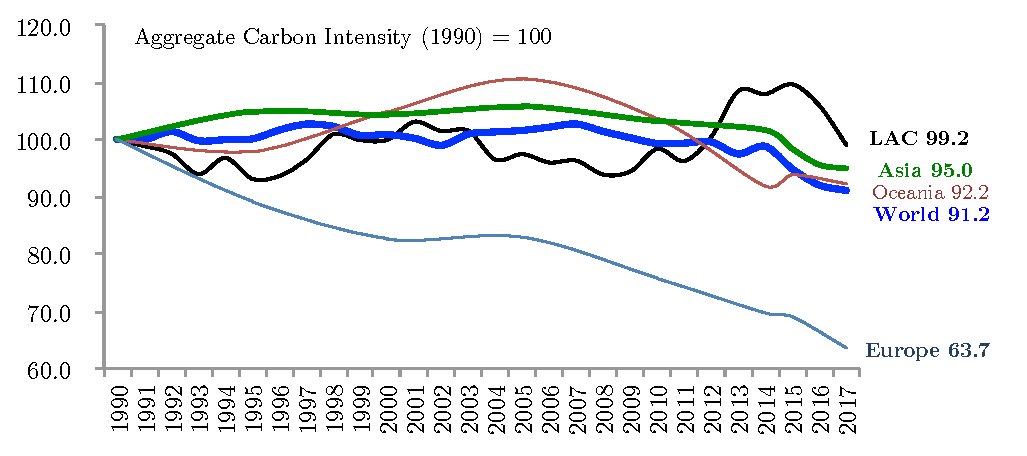
\includegraphics[width=13cm]{images/globACI.pdf}}
       \caption{Change of aggregate carbon intensity for electricity, period 1990-2017, (1990=100) \cite{IEAEnergyCombution2019}}
      \label{globACI}
        \end{figure}

Notice that since 1990 the ACI of Europe, Oceania, Asia and the World have dropped about 37.3 \%, 7.8 \%, 5.0 \%  and 8.8 \%, respectively.  Instead, the ACI of Latin-American countries are showing a small decrease of 0.8 \%. We must to highlight that the regional ACI index has showed high variability as can be observed in Fig.  \ref{globACI}, mainly in the last three years when the indicator fell from 285 gCO$_2$/kWh in 2015 to 257.7 gCO$_2$/kWh. This changing trend justifies focusing on the LAC electricity sector as it is expected to be an important contributor to the mitigation effort due to its large renewable resources.


Statistical decomposition techniques have been widely applied in literature to analyze total carbon dioxide emission  time-series \cite{zhang2000}.   A survey on IDA-LMDI analyses applied to decompose total CO$_2$ emissions can be found in \cite{zhang2000}. A more recent review includes 17 publications that use IDA to study CO$_2$ emissions of the electricity sector \cite{xu2013}. Some recent publications in this topic can be find out. New IDA-LMDI analyses have been carried out in the U.S \cite{jiang}, China \citep{zhao}, the European Union \cite{zkar}, Philippine \cite{sum} and Greece \cite{dia} electricity generation sectors.

 However, we can observe that few contributions are devoted to analyzed carbon intensity time-series using statistical decomposition techniques. We would like to emphasize that carbon dioxide magnitudes in million tonnes of CO$_2$ and carbon dioxide intensities  in gCO$_2$/kWh are different concepts. Further discussion about the key differences between both concepts are provided in \cite{ang2016}.
 
  The IDA-LMDI procedures applied to ACI decomposition are scarce in Liteature as shown in Table \ref{tableLMDI0}. The methodology is general and it can be applied for any country or region of the world using either a single-period or a multi-temporal scope. Existing contributions on IDA-LMDI decomposition of ACI time-series are based on a single period, i.e. 1990-2017. The main drawback of the single-period approach is that the drivers behind ACI variability are difficult to capture. Under a multi-temporal decomposition approach different accelerating and and attenuating drivers of the ACI behavior, as showed in Figure   \ref{globACI}, can be analyzed considering a number of periods.
 
 The IDA-LMDI methodology has been applied to decompose global \cite{ang2016} and Asean  \cite{goh} carbon intensity time-series for 1990-2012 and 1990-2013, respectively. The carbon intensity of different regions of China's power sector has been analyzed in \cite{peng, liu,liu2}. Recently, the authors \cite{oliv} have analyzed the effect of the generation system capacity factor using an LMDI formulation in Latin America and the Caribbean considering a single period 1990-2014. 

		\begin{table}[!ht]													
		\begin{center}\caption{IDA-LMDI analysis applied to ACI time-series}													
		\begin{tabular}{lcccc}\hline				Reference	&	Region	&	Single-Period	& Multi-period 	\\	\hline
		Ang (2016)	\cite{ang2016} 	&	World	&	$\circ$	&		 	\\
		Ang (2016)	\cite{goh} 	&	Asia	&	$\circ$	&		 	\\
		Peng (2018)	\cite{peng} 	&	China	&	$\circ$	&			\\
				Liu (2017)	\cite{liu} 	&	China	&	$\circ$	& 			\\
		Liu (2019)	\cite{liu2} 	&	China	&	$\circ$	& 			\\
		De Oliveira-De Jesus (2019)	\cite{oliv} &	LAC 	&   $\circ$ &	 		\\ 

		This paper &	LAC 	&   &	 	 $\circ$	\\
		\hline
		\end{tabular}\label{tableLMDI0}	
		\end{center}				
		\end{table}							


After carefully review of literature, it was not found any detailed IDA-LMDI analysis related with the evolution of electricity generation sector of Latin American and Caribbean countries under a multi-period basis.
   To fulfill the research gap, this paper develops a Logarithmic Mean Divisia Index (LMDI) method of complete decomposition to determine the key factors behind the evolution of ACI from electricity generation in Latin American countries. The proposed analysis expressly includes the effect of each country and fuel-type used in thermal plants in the evolution of the regional ACI.  Results are discussed in the context of country-specific energy policies adopted to cope the environmental challenges.

This the paper is organized as follows. Section \ref{sec3} presents the time-series related to the ACI of Latin-America countries to be analized. Section \ref{sec4} describes
the IDA-LMDI methodology applied. Results are presented in Section \ref{sec5}. Some implications of the results are discussed in Section \ref{policy}. Finally, conclusions are drawn in Section \ref{sec7}.



\section{Latin-America aggregated CO$_2$ emission intensities}  \label{sec3}

According to the IEA, the global electricity production increased from 623.2 TWh per year in 1990 to 1614 TWh per year in 2017 \cite{IEAEnergyCombution2019}.  On the other hand, the associated CO$_2$ emissions also increased from 161 to 416 MtCO$_2$ per  year in the same period  \cite{IEAEnergyCombution2019}. Given the annual emissions and total annual electricity generation output from 1990 to 2017, we can also determine the annual Aggregate Carbon Intensity (ACI) for electricity of Latin America \& the Caribbean over a 28-year time span.


\begin{figure}[h!]
	\begin{center} 
	    \centering
		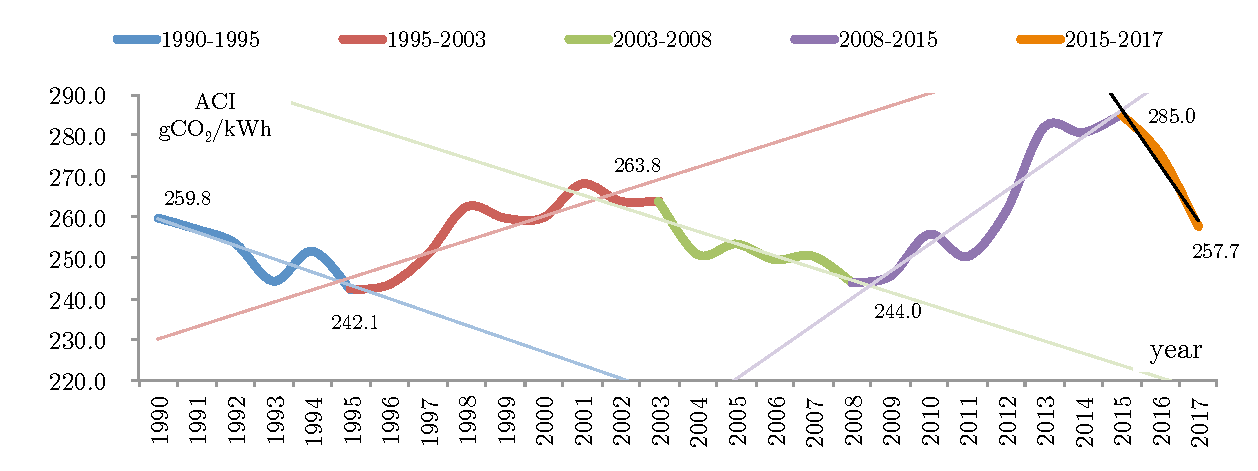
\includegraphics[width=13cm]{images/plot.pdf}
		\caption{The aggregate carbon intensity of Latin-America, 1990-2017} 
		\label{plot1}
		\end{center} 
\end{figure}


Figure \ref{ACI2} shows how the regional carbon intensity have ranged from 259.8 gCO$_2$/kWh in 1990 to 257.7  gCO$_2$/kWh in 2017. A
decrease of 2.2 gCO$_2$/kWh or -0.8\% of the 1990 level over the
period is observed. Note that over a 28-year time span,  five different accelerating and attenuating periods can be identified. Two increasing periods (1995-2003, 2008-2015) and three declining periods (1990-1995, 2003-2008, 2015-2017).


              \begin{figure}[ht] \centerline{
     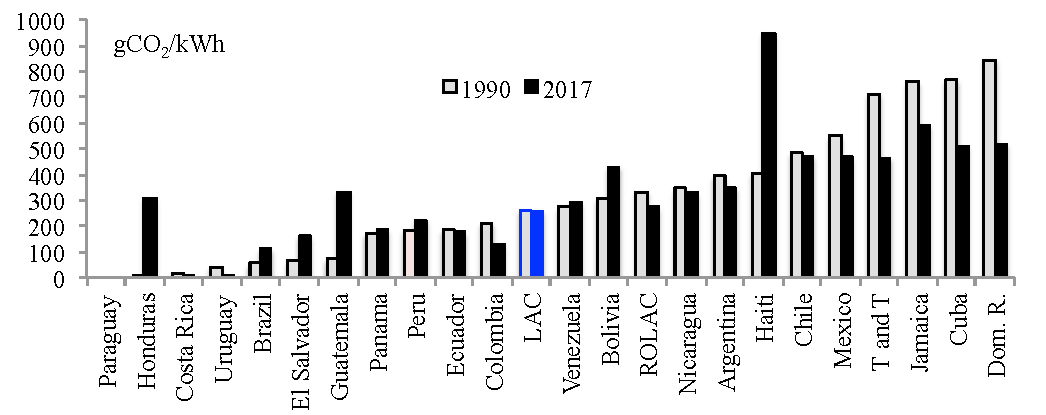
\includegraphics[width=12cm]{images/ACIpercounry.pdf}}
       \caption{The aggregate carbon intensity by LAC country,  1990-2017}
      \label{ACIpercounry}
        \end{figure}
        
        
          The estimated levels of carbon dioxide emissions associated with the power sector are different in each country of the region. The changes in the ACI between 1990 and 2017 by each country are presented in Figure  \ref{ACIpercounry}.
This figure shows the most representative countries. The remaining countries of the Latina-America region are grouped as the "rest of LAC countries" (ROLACs). It is observed that larger electricity producers as Brazil, Ecuador, Peru and Bolivia have significantly increased their carbon intensity between 1990 and 2017 but below the regional average by 2017 (257.7 gCO$_2$/kWh). Other important producers as Mexico, Argentina, Chile, Colombia have reduced their carbon intensity with respect to the average values. Notice that small countries such as Honduras, Guatemala and Haiti are showing important increases in their carbon intensity.

 The carbon intensity of the biggest electricity producer of the region (Brazil) increased from 55 gCO$_2$/kWh in 1990 to
113 gCO$_2$/kWh in 2017. It must be noted that both values are moderate with respect to the average values of LAC in 1990 (259.8 gCO$_2$/kWh) and 2017 (257.7 gCO$_2$/kWh), figures depicted with blue bars in Figure \ref{ACIpercounry}.  


The second electricity producer of the region  (Mexico) decreased their carbon intensity from 549 gCO$_2$/kWh in 1990 to 471 gCO$_2$/kWh in 2017. In this case both values clearly exceed the average values in both years. Most relevant reductions are achieved in Colombia, Uruguay and some Caribbean islands as Cuba, Jamaica, Trinidad \& Tobago and Dominican Republic. Argentina, Venezuela, Cuba and Nicaragua remains stable and as Paraguay has a 100\% renewable power sector no emissions are assigned to this country.




To account for the impact of all countries electricity production  levels, the carbon intensity figures depicted in Figure \ref{ACIpercounry} for 1990 and 2017 are resettled in descending order and plotted against the cumulative electricity production. This exercise was previously performed by  \cite{ang2016} using world carbon intensity evolution from 1990 to 2014. The resulting chart for the Latin-America case is depicted in Figure \ref{cumglobACI}. 

               \begin{figure}[ht] \centerline{
     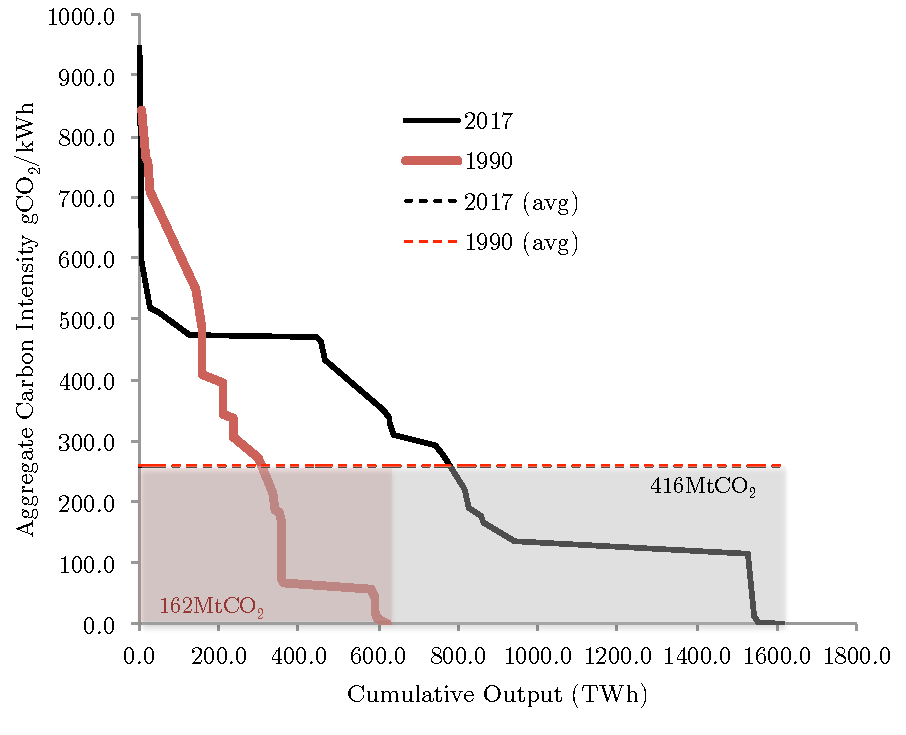
\includegraphics[width=10cm]{images/cumglobACI.pdf}}
       \caption{Carbon intensity vs cumulative electricity production in LAC,  1990-2017}
      \label{cumglobACI}
        \end{figure}

The cumulative curves are depicted as solid lines with different colors, red for 1990 and black for 2017, respectively. 
The 2017 cumulative curve stretches further to the right on the horizontal axis since the total electricity production in 2017 was about three times the level registered in 1990. The area below both cumulative curves represent the global CO$_2$ emissions from electricity production in the year given in MtCO$_2$. The 1990 and 2017 total average ACI values change from 259.8 to 257.7 gCO$_2$/kWh being represented by two horizontal
 dashed lines. Note that the range of the carbon intensity values in the vertical axis is almost the same for both years. 
For each specific year, the difference
between the solid cumulative curve and the horizontal dashed lines provides
an indication of the changes for each ACI at country level.
with respect to the total weight average. In Figure \ref{cumglobACI}, the shadowed rectangle enclosed by the dashed lines
 provides the equivalent
total CO$_2$ emissions for 1990 and 2017.  The two rectangles exemplifies how the
 total electricity production, average ACI, and
 total CO$_2$ emissions have changed over the period.
 It means that despite almost
a tripling in total electricity production and CO$_2$ emissions from 1990 to 2017 the average ACI
fell about 0.8 \%.
	
																						
\section{Methodology}  \label{sec4}

Laspeyres index and Divisia index decomposition procedures are   frequently used to perform analytics in energy and environmental studies \cite{zhang2000}. The decomposed driving factors are associated with certain variables that explain the evolution of a variable of interest, i.e. the aggregate carbon intensity for electricity. In their original formulation, Laspeyres index and Divisia methods produce  a residual factor that is difficult to explain \cite{angperfect}. The IDA-LMDI method proposed by \cite{angperfect} eliminates the residual term by means of a perfect decomposition.



In a specific year, Eq. \ref{ldmi1} expresses the total annual  CO$_2$ emissions from electricity as function of a series of variables (input time-series) \cite{ang2016}.

\begin{equation}\label{ldmi1}
  C=\sum^n_{j=1}	C_{j}=\sum^n_{j=1}\sum^f_{i=1}\frac{C_{ij}}{F_{ij}}
  \frac{F_{ij}}{Q_{ij}} \frac{Q_{ij}}{Q_{j}} \frac{Q_{j}}{G_{j}} \frac{G_{j}}{G} G
\end{equation}


where:

$n$ is the number of countries under analysis

$f$ is the number of fossil fuel types. Three fossil fuel types are considered: coal ($i$=1),  natural gas ($i$=2) and   oil products ($i$=3)

$C_{ij}$ is the electricity-related CO$_2$ emissions from fossil fuel $i$ in country $j$  [kt CO$_2$]

$C_{j}$ is the electricity-related CO$_2$ emissions in country $j$ [kt CO$_2$]. Note that $C_{j}=\sum_{i=1}^f C_{ij}$.



$F_{ij}$ is energy input from fossil fuel $i$ in country $j$ [TWh]

$Q_{ij}$ is the electricity output from fossil fuel $i$ in country $j$ [TWh]

$Q_{j}$ is the electricity output from fossil fuels in country $j$ [TWh]. Note that $Q_{j}=\sum_{i=1}^f Q_{ij}$

$G_{j}$ is the  electricity output (fossil and renewable) in country $j$ [TWh].  Note that $G=\sum_{j=1}^n G_{j}$.


 Three decomposition properties can be identified in the IDA equation \ref{ldmi1}: (a) the total electricity output $G$ is the main "activity" that produces CO$_2$ emissions, (b) proportions
${Q_{ij}}/{Q_{j}}$, ${Q_{j}}/{G_{j}}$ and  ${G_{j}}/{G}$ indicate "structural" factors related with the share of the different fuel types in the national fossil-based electricity production, the share of fossil-based production in the national electricity production and the share of national production with respect to the total electricity output, (c) proportions ${C_{j}}/{F_{ij}}$ and ${F_{ij}}/{Q_{ij}}$ provides information about the "intensity" of  each fuel type in local emissions and the efficiency of each generating plant fuel type, respectively. As made in the basic approach,  total CO$_2$ emissions should be normalized for kWh produced  to obtain the ACI index, then Equation \ref{ldmi1} can be rewritten as \cite{ang2016}:

 \begin{equation}\label{ldmi2}
  V=\frac{C}{G}=\sum^n_{j=1}\sum^f_{i=1} {e_{ij}}  {u_{ij}}  {m_{ij}} {p_{j}} {s_{j}} =
  {I_{ij}}{S_{j}}
\end{equation}

\noindent where following driving factors are defined:

\noindent $e_{ij}=C_{ij}/F_{ij}$ is the CO$_2$ intensity factor of fossil fuel $i$ for a country $j$ [gCO$_2$/kWh].

\noindent $u_{ij}=F_{ij}/Q_{ij}$ is the thermal heat rate of fossil-fired plants with fuel $i$ for a country $j$.

\noindent $m_{ij}=Q_{ij}/Q_{j}$ is the fuel $i$ share of electricity d from fossil  fuels for a country $j$.

\noindent $p_{j}=Q_{j}/G_{j}$ is the fossil share of electricity for a country $j$.

\noindent $s_{j}=G_{j}/G$ is the electricity production for a country $j$ as a share of
total electricity production.

The IDA identity \ref{ldmi2} is then characterized by five factors, two structural factors (${S_{j}}$=$s_{j} \times p_{j}$ ) and three intensity factors
(${I_{ij}}= e_{ij} \times u_{ij} \times m_{ij}$). Then ${S_{j}}$ and ${I_{ij}}$ denote the structural and intensity drivers, respectively.



The IDA-LMDI can be applied into two different formulations: additive decomposition analysis and
multiplicative decomposition analysis \cite{zhang2000}. Both methods provide the same insight about the impact or effect of each
driving factor at a given time frame. On one hand, under the additive approach, the effect of a given driving factor is explained through an arithmetic value that may positive or negative. On the other hand, under the multiplicative approach, the  effect is expressed as a proportion of the initial value of the dependent variable. Both approaches allow us to visualize in different ways what happened with these drivers in the period under study.






Next subsections are devoted to present additive and multiplicative IDA-LMDI formulations in detail. 

\subsection{Additive IDA-LMDI decomposition method}\label{amm1}


Under the additive IDA-LMDI approach the arithmetic change in total ACI
$\Delta V$ from year $t_f$ to year $t_0$ can then be decomposed to give \cite{ang2016}:

\begin{equation}\label{dvtot}
  \Delta V   =  V^{t_f}- V^{t_0} = \Delta V_{e} + \Delta V_{u}+
  \Delta V_{m} + \Delta V_{p}  + \Delta V_{s} = \Delta V_{int}+\Delta V_{str}
\end{equation}

\noindent where $\Delta V_{e}$, $\Delta V_{u}$, $\Delta V_{m}$, $\Delta V_{p}$  and $\Delta V_{s}$ reproduce the effects between from ${t_f}$ and ${t_0}$ associated with variations in $e_{ij}$, $u_{ij}$, $m_{ij}$, $p_{j}$ and $s_{j}$, respectively.   The meanings of these effects are as follows. The "CO$_2$ intensity of the fuel-mix effect" $\Delta V_{e}$, the "generation efficiency effect" $\Delta V_{u}$ and the "fossil-share of electricity effect" $\Delta V_{p}$ were previously defined in the basic approach. This detailed model requieres to define other two drivers in order to capture the effect of fuels and countries.  The first one is the "fossil fuel-mix effect" $\Delta V_{m}$ that expresses the  changes in the mix of fossil fuels used to produce fossil-based electricity (share of fossil-based electricity). The second one is the "geographical shift effect" $\Delta V_{s}$ that expresses  changes in electricity output for a specific country with respect to total electricity output (all LAC countries).

Furthermore, the "intensity effect" and the "structural effect" denote the impact of the fuel-mix ($\Delta V_{int}$=$\Delta V_{e} + \Delta V_{u}+ \Delta V_{m}$) and the fossil-share in a country and total electricity output ($\Delta V_{str}$= $  \Delta V_{p}  + \Delta V_{s}$), respectively.  The corresponding decomposition IDA-LMDI formulae for the additive approach is included in the Appendix \ref{app1}.

\subsection{Multiplicative IDA-LMDI decomposition method}\label{amm2}

 Under the multiplicative IDA-LMDI approach the proportional change in total ACI
$U$ from year $t_f$ to year $t_0$ is decomposed to give \cite{ang2016}:

\begin{equation}
  U   = \frac{ V^{t_f}}{ V^{t_0}} = U_{e} U_{u} U_{m} U_{p} U_{s} = U_{int}U_{str}
\end{equation}

where $U_{e}$, $U_{u}$,  $U_{p}$  and $U_{s}$ are respectively the effects associated with variations in $e_{ij}$, $u_{ij}$,  $m_{ij}$, $p_{j}$ and $s_{j}$, respectively. The meanings of these effects are as follows.

The "CO$_2$ intensity of the fuel-mix effect" $U_{e}$, the "generation efficiency effect" $U_{u}$ and the "fossil-share of electricity effect" $U_{p}$ were previously defined in the basic approach.  The "fossil fuel-mix effect" $U_{m}$ the "geographical shift effect" $U_{s}$ expresses proportional changes in the fuel-mix of electricity as well as the share total electricity production.

In the same way that in the additive form, the "intensity effect" measures the impact of fuel-mix in the emissions produced in all thermal power stations: $U_{int}$=$U_{e}   U_{u}  U_{m}$. The "structural effect" indicates the change of the fossil-share of the total electricity.  The value of the structural effect is given by $U_{str}$= $  U_{p}   U_{s}$. The corresponding decomposition IDA-LMDI formulae for the multiplicative approach is included in the Appendix \ref{app2}.



\section{Results and Analysis}  \label{sec5}


The additive and multiplicative IDA-LMDI method has been applied to characterize the evolution of the regional aggregate carbon intensity of electricity encompassing all Latin America \& the Caribbean countries. Besides the decomposition analysis for the main period 1990-2017, as a key contribution of this paper, the decomposition method has been applied under a multi-temporal basis considering five periods defined from Figure \ref{plot1} as follows:

\begin{enumerate}
  \item 1990-1995 when the ACI changed (decreased) from 259.8 to 242.1 gCO$_2$/kWh
  \item 1995-2003 when the ACI changed (increased) from 242.1 to 263.8 gCO$_2$/kWh
  \item 2003-2008 when the ACI changed (decreased) from 263.8 to 244.0 gCO$_2$/kWh
  \item 2008-2015 when the ACI changed (increased) from 244.0 to 286.0 gCO$_2$/kWh
  \item 2015-2017 when the ACI changed (decreased) from 286.0 to 257.7 gCO$_2$/kWh
\end{enumerate}

The interested reader can replicate the results reported below by assessing the following GitHub web page: https://github.com/pmdeoliveiradejesus/LMDI-LatinAmerica/

\subsection{Data sources and assumptions} \label{basicres}

Latin America \& the Caribbean region is made up of 51 countries\footnote{Latin American \& the Caribbean countries comprise: Argentina; Bolivia; Brazil; Chile
Colombia; Costa Rica; Cuba;  the Dominican
Republic; Ecuador; El Salvador; Guatemala; Haiti;
Honduras; Jamaica; Mexico, Nicaragua; Panama; Paraguay;
Peru; Suriname, Trinidad and Tobago;
Uruguay; Venezuela and other small Caribbean countries as Antigua and
Barbuda; Aruba; the Bahamas; Barbados; Belize;
Bermuda; Bonaire; the British Virgin Islands;
the Cayman Islands; Curacao; Dominica; the Falkland Islands
(Malvinas); the French Guiana; Grenada; Guadeloupe;
Guyana; Martinique; Montserrat; Puerto Rico; Saba; Saint
Eustatius; Saint Kitts and Nevis;
Saint Lucia; Saint Pierre and Miquelon; Saint Vincent
and the Grenadines; Saint Maarten and the Turks and Caicos Islands.}. Time-series of 22 countries that contribute most to the region's CO$_2$ emissions are considered: Argentina, Bolivia, Brazil, Chile, Colombia,
 Costa Rica, Cuba, Dominican Republic, Ecuador, El Salvador, Guatemala, Haiti, Honduras, Jamaica, Mexico, Nicaragua, Panama, Paraguay,
 Peru, Trinidad and Tobago, Uruguay and Venezuela. The remaining 29 countries in the dataset only represent 2.4 \% of total emissions by 2017. These remaining countries are grouped together as a single entity referred to as the "rest of LAC countries" (ROLACs). Accordingly a total 22 countries plus the equivalent country called ROLAC are considered in the  decomposition analysis.
 
 
The energy and environmental dataset of $j$=1,...,23 countries are taken from the IEA's internet  public database (https://www.iea.org/data-and-statistics/data-tables). Last year available is 2017. Three fossil fuel types are considered: coal ($i$=1),  natural gas ($i$=2) and   oil products ($i$=3). Four time series 1990-2017 are required to apply the methodology: 

\begin{enumerate}
  \item $C_{ij}$: electricity-related CO$_2$ emissions from fossil fuel $i$ in country $j$  [Mt CO$_2$].

\item $F_{ij}$: energy input from fossil fuel $i$ in country $j$ [TWh]. 

\item $Q_{ij}$: electricity output from fossil fuel $i$ in country $j$ [TWh] and,  

\item $G_{j}$: electricity output (fossil and renewable) in country $j$ [TWh].
\end{enumerate}



 The interested reader can request to the authors the dataset in order to replicate the results of the paper using the method described in Section \ref{sec4}.   

 \subsection{The additive IDA-LMDI analysis results} \label{addres}

 The additive IDA-LMDI decomposition approach presented in Section \ref{amm1} is applied. The  additive decomposition approach is performed according to Eq. \ref{dvtot} using Eq. \ref{dvtot1}-\ref{dvtot5} of the  \ref{app1}. General results over the main period 1990-2017 and for the five periods (1990-1995, 1995-2003, 2003-2008, 2008-2015 and 2015-2017) are presented in Table \ref{table1}. All figures of the table are given in gCO$_2$/kWh.
 

\begin{table}[!h]\label{11}										
\begin{center}\caption{Additive LMDI-IDA analysis results (gCO$_2$/kWh)}			
\begin{tabular}{l|c|cc|ccc|cc}\hline	
Period	 &$	\Delta V	$&$	\Delta V_{int}	$&$	\Delta V_{str}$	&$	\Delta V_e	$&$	\Delta V_{u}	$&$	\Delta V_{m}	$&$	\Delta V_{p}	$&$	\Delta V_{s}	$		\\\hline
1990-2017	&	-2.1	&\textcolor{red}{\textbf{	-66.9	}}&\textcolor{blue}{\textbf{	64.7	}}&	-5.3	&\textcolor{red}{\textbf{	-36.0	}}&	-25.6	&\textcolor{blue}{\textbf{	63.1	}}&	1.6	 	\\\hline
1990-1995	&	-17.7	&\textcolor{red}{\textbf{	-14.1	}}&	-3.6	&\textcolor{red}{\textbf{	-6.7	}}&\textcolor{red}{\textbf{	-4.7	}}&	-2.7	&	-4.5	&	0.9	 \\
1995-2003	&	21.8	&	-26.8	&\textcolor{blue}{\textbf{	48.6	}}&	-6.8	&	-6.0	&	-13.9	&\textcolor{blue}{\textbf{	40.7	}}&	7.8	 \\
2003-2008	&	-19.9	&\textcolor{red}{\textbf{	-28.4	}}&	8.5	&	-13.0	&\textcolor{red}{\textbf{	-16.0	}}&	0.6	&	11.1	&	-2.5	 \\
2008-2015	&	41.0	&	6.2	&\textcolor{blue}{\textbf{	34.8	}}&	5.4	&	-4.7	&	5.5	&\textcolor{blue}{\textbf{	35.4	}}&	-0.6	 \\
2015-2017	&	-27.4	&\textcolor{red}{\textbf{	-9.2	}}&\textcolor{red}{\textbf{	-18.2	}}&	3.0	&\textcolor{red}{\textbf{	-10.6	}}&	-1.6	&\textcolor{red}{\textbf{	-18.4	}}&	0.2 \\\hline
\end{tabular}\label{table1}										
\end{center}										
\end{table}	



The first column of Table \ref{table1} lists the periods of study. The second column includes the total changes of ACI ($\Delta V$)  for each period.  Next two columns in the table account the structural and intensity effects ($\Delta V_{str}$ and $\Delta V_{int}$)  for each period. The structural  driver corresponds to the sum of the fuel-share in the electricity output and the geographical effects  ($\Delta V_{str}$=$\Delta V_{p}$+$\Delta V_{s}$). The intensity driver  corresponds to the sum of the emission , efficiency and fuel-mix effects  ($\Delta V_{int}$=$\Delta V_{u}$+$\Delta V_{e}$+$\Delta V_{m}$). The intensity driver  associated with the carbon emission intensity ($\Delta V_{e}$) and  efficiency ($\Delta V_{u}$) as well as
the structural effect  associated with fuel-share of electricity ($\Delta V_{p}$) were also decomposed by fuel type and presented in Table \ref{table2}. 





\begin{table}[!h]\label{11}										
\begin{center}\caption{The additive LMDI-IDA analysis results by fuel type in all periods (gCO$_2$/kWh)}			
\begin{tabular}{l|cccc|cccc|cccc}\hline	
 	&\multicolumn{4}{c|}{emission effect}	&\multicolumn{4}{c|}{efficiency effect}	 	&\multicolumn{4}{c}{fuel mix effect}		\\ 
 	Period	&$	\Delta V_e	$&$	\Delta V_{e1}	$&$	\Delta V_{e2}	$&$	\Delta V_{e3}	$&$	\Delta V_{u}	$&$	\Delta V_{u1}	$&$	\Delta V_{u2}	$&$	\Delta V_{u3}	$&$	\Delta V_{m}	$&$	\Delta V_{m1}	$&$	\Delta V_{m2}	$&$	\Delta V_{m3}$	\\ 
 	& fossil	 &	coal	&	gas	&	oil	&	fossil  	&	coal	&	gas	&	oil	&	fossil 	& coal	 &	gas	&	oil		\\\hline
1990-2017	&	-5.3	&	0.0	&	-0.4	&	-4.9	&	\textcolor{red}{\textbf{-36.0}}	&	-6.6	&	\textcolor{red}{\textbf{-16.5}}	&	-12.8	&	-25.6	&	-5.0	&	68.1	&	-88.7	\\\hline
1990-1995	&	\textcolor{red}{\textbf{-6.7}}	&	0.0	&	-0.3	&	\textcolor{red}{\textbf{-6.4	}}&	\textcolor{red}{\textbf{-4.7	}}&	-1.3	&	\textcolor{red}{\textbf{-4.7}}	&	1.2	&	-2.7	&	8.9	&	9.1	&	-20.6	\\
1995-2003	&	-6.8	&	0.0	&	0.0	&	-6.8	&	-6.0	&	3.6	&	-6.1	&	-3.6	&	-13.9	&	-12.7	&	32.0	&	-33.3	\\
2003-2008	&	-13.0	&	0.0	&	0.0	&	-13.0	&	\textcolor{red}{\textbf{-16.0}}	&	-1.3	&	-5.6	&	\textcolor{red}{\textbf{-9.2}}	&	0.6	&	-7.7	&	9.0	&	-0.7	\\
2008-2015	&	5.4	&	0.0	&	0.0	&	5.4	&	-4.7	&	-4.0	&	-1.5	&	0.8	&	5.5	&	13.2	&	10.1	&	-17.9	\\
2015-2017	&	3.0	&	0.0	&	0.0	&	3.0	&	\textcolor{red}{\textbf{-10.6}}	&	-2.4	&	-0.9	&	\textcolor{red}{\textbf{-7.2}}	&	-1.6	&	0.3	&	6.0	&	-7.9	\\\hline
\end{tabular}\label{table2}										
\end{center}										
\end{table}

         Some additional notation is necessary to highlight the results enclosed in the tables. In order to indicate the most important effects that contribute to actual trend of the ACI table entries are highlighted in bold blue between squared brackets. Conversely, most important effects that do not contribute (mitigate) to actual trend are highlighted in bold red between round brackets.
        



        
        

        
   Figure  \ref{main1} also displays a graph representation of results presented in Table \ref{table1}. The
solid circles depicted in Figure  \ref{main1} over each period bar representation also indicate the total ACI changes ($\Delta V$).

%                             \begin{figure}[!h] \centerline{
%     \includegraphics[width=8cm]{images/main4.pdf}}
%       \caption{Change of ACI (gCO$_2$/kWh) in all periods - Results by Country}
%      \label{main4}
%        \end{figure}

%

        \begin{figure}[H] \centerline{
       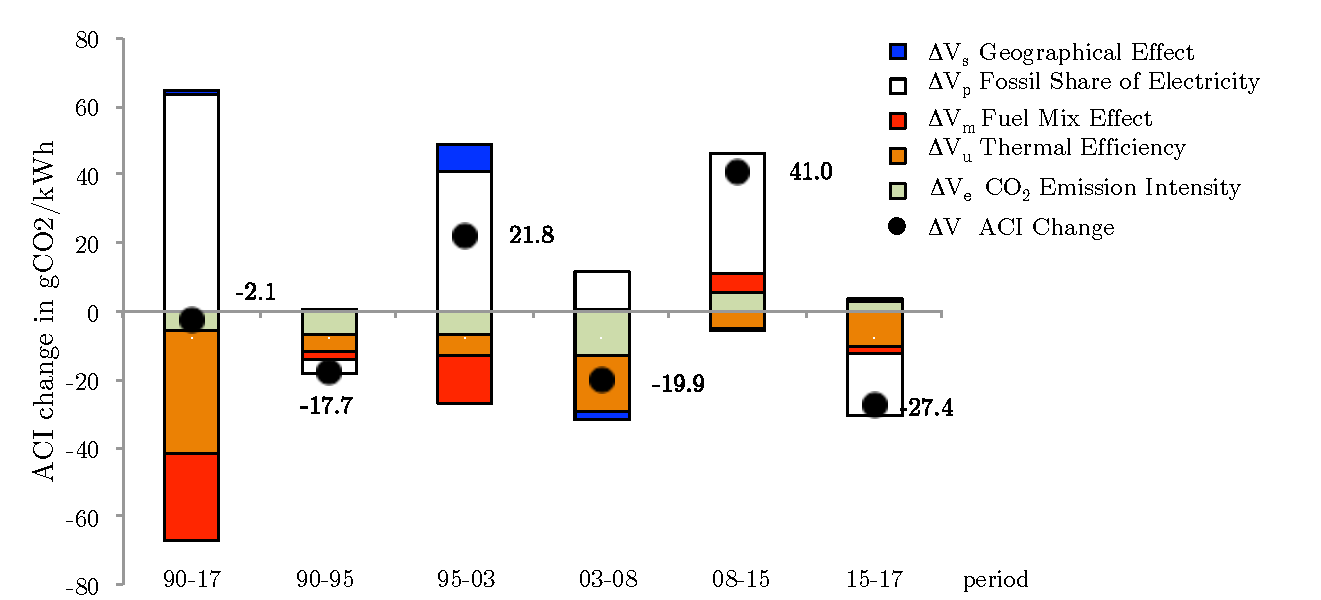
\includegraphics[width=15cm]{images/Figura4.pdf}}
       \caption{Additive LMDI-IDA analysis applied to CO$_2$ emissions considering 5 periods (gCO$_2$/kWh)}
      \label{main1}
        \end{figure}
        
        
We can observe the following general results in each period:

\begin{itemize}
  \item 1990-2017 the ACI changed (decreased) from 259.8 to 257.7 gCO$_2$/kWh due to INTENSITY reasons (improvements in  gas-fired plant efficiency).
  \item 1990-1995 the ACI changed (decreased) from 259.8 to 242.1 gCO$_2$/kWh due to INTENSITY reasons (improvements in  fuel-fired plant efficiency).
  \item 1995-2003 the ACI changed (increased) from 242.1 to 263.8 gCO$_2$/kWh due to STRUCTURAL reasons (fossil-share increase)
  \item 2003-2008 the ACI changed (decreased) from 263.8 to 244.0 gCO$_2$/kWh due to INTENSITY reasons (improvements in  coal-fired plant efficiency).
  \item 2008-2015   the ACI changed (increased) from 244.0 to 286.0 gCO$_2$/kWh due to STRUCTURAL reasons (fossil-share increase)
  \item 2015-2017 when the ACI changed (decreased) from 286.0 to 257.7 gCO$_2$/kWh  due to INTENSITY reasons (improvements in  coal-fired plant efficiency and decrease of fossil-share).
\end{itemize}

In the following, we will analyze these overall results considering the intensity and structural drivers obtained by country.

\newpage



\subsubsection{Period 1990-2017}

 Specific results of intensity and structural  drivers by country for the main period 1990-2017 are presented in Table \ref{table3}.

  \begin{table}[!h]\label{11}										
\begin{center}\caption{Additive LMDI-IDA analysis applied to CO$_2$ emissions by country 1990-2017}			
\begin{tabular}{l|c|c:c|ccc:cc}\hline	
Country	&$	\Delta V  	$&$	\Delta V_{int}	$&$	\Delta V_{str}	$&$	\Delta V_{e}	$&$	\Delta V_{u}	$&$	\Delta V_{m}	$&$	\Delta V_{p}	$&$	\Delta V_{s}	$\\\hline										
Argentina	&	-0.52	&	-12.49	&	11.97	&	-0.79	&	-10.01	&	-1.70	&	8.74	&	3.23	\\																					
Bolivia	&	1.52	&	-0.13	&	1.65	&	2.76	&	0.00	&	-2.89	&	0.77	&	0.88	\\																					
Brazil	&	21.83	&	-14.19	&	36.02	&	-0.18	&	-7.95	&	-6.07	&	35.49	&	0.53	\\																					
Chile	&	8.95	&	-3.61	&	12.56	&	-0.15	&	-2.05	&	-1.41	&	3.46	&	9.10	\\																					
Colombia	&	-5.93	&	-3.05	&	-2.88	&	0.05	&	-1.46	&	-1.64	&	-1.31	&	-1.58	\\																					
Costa Rica	&	-0.11	&	-0.04	&	-0.07	&	-0.03	&	-0.01	&	0.00	&	-0.07	&	0.01	\\																					
Cuba	&	-11.94	&	-5.67	&	-6.27	&	-0.24	&	-4.78	&	-0.65	&	0.76	&	-7.03	\\																					
Dom. Rep.	&	1.12	&	-0.86	&	1.98	&	-0.08	&	-1.49	&	0.71	&	-1.25	&	3.23	\\																					
Ecuador	&	1.31	&	-0.76	&	2.07	&	-0.05	&	-0.55	&	-0.16	&	0.74	&	1.33	\\																					
El Salvador	&	0.32	&	-0.16	&	0.48	&	0.01	&	-0.17	&	0.00	&	0.50	&	-0.02	\\																					
Guatemala	&	2.44	&	0.99	&	1.45	&	-0.04	&	-1.57	&	2.60	&	0.88	&	0.57	\\																					
Haiti	&	0.23	&	-0.30	&	0.53	&	0.01	&	-0.31	&	0.00	&	0.72	&	-0.19	\\																					
Honduras	&	1.76	&	0.17	&	1.59	&	0.01	&	0.09	&	0.07	&	1.40	&	0.19	\\																					
Jamaica	&	-1.38	&	-0.03	&	-1.34	&	0.21	&	-0.24	&	0.00	&	-0.51	&	-0.83	\\																					
Mexico	&	-8.05	&	-22.64	&	14.59	&	-5.63	&	-3.07	&	-13.94	&	8.63	&	5.96	\\																					
Nicaragua	&	0.06	&	-0.20	&	0.26	&	0.01	&	-0.21	&	0.00	&	0.16	&	0.10	\\																					
Panama	&	0.57	&	-0.50	&	1.07	&	-0.05	&	-0.50	&	0.05	&	0.62	&	0.45	\\																					
Paraguay	&	0.00	&	0.00	&	0.00	&	0.00	&	0.00	&	0.00	&	0.00	&	0.00	\\																					
Peru	&	3.18	&	-0.49	&	3.67	&	-0.19	&	0.50	&	-0.79	&	2.16	&	1.51	\\																					
T \& T	&	-0.91	&	-1.56	&	0.65	&	0.00	&	-1.56	&	0.00	&	0.02	&	0.63	\\																					
Uruguay	&	-0.40	&	0.03	&	-0.43	&	0.02	&	0.01	&	0.00	&	-0.34	&	-0.09	\\																					
Venezuela	&	-6.78	&	0.33	&	-7.11	&	0.70	&	-0.63	&	0.25	&	1.21	&	-8.32	\\																					
ROLAC	&	-9.41	&	-1.68	&	-7.73	&	-1.69	&	0.00	&	0.00	&	0.34	&	-8.07	\\\hline																					
Total	&	-2.15	&	-66.85	&	64.70	&	-5.34	&	-35.95	&	-25.56	&	63.12	&	1.58																															
\end{tabular}	\label{table3}									
\end{center}										
\end{table}	

The most important mitigating effect on the ACI change between 1990-2017 is attributable to Cuba and Mexico: $\Delta V^{cub}$=-11.9 gCO$_2$/kWh and   $\Delta V^{mex}$=-8.0 gCO$_2$/kWh. The most important accelerating effect on the ACI change between 1990-2017 is attributable to Brazil: $\Delta V^{bra}$=-+21.8 gCO$_2$/kWh. 

Figure \ref{countriesPlot} shows the contribution of all LAC countries from intensity and structural views.  

        \begin{figure}[H]
	\begin{center} 
		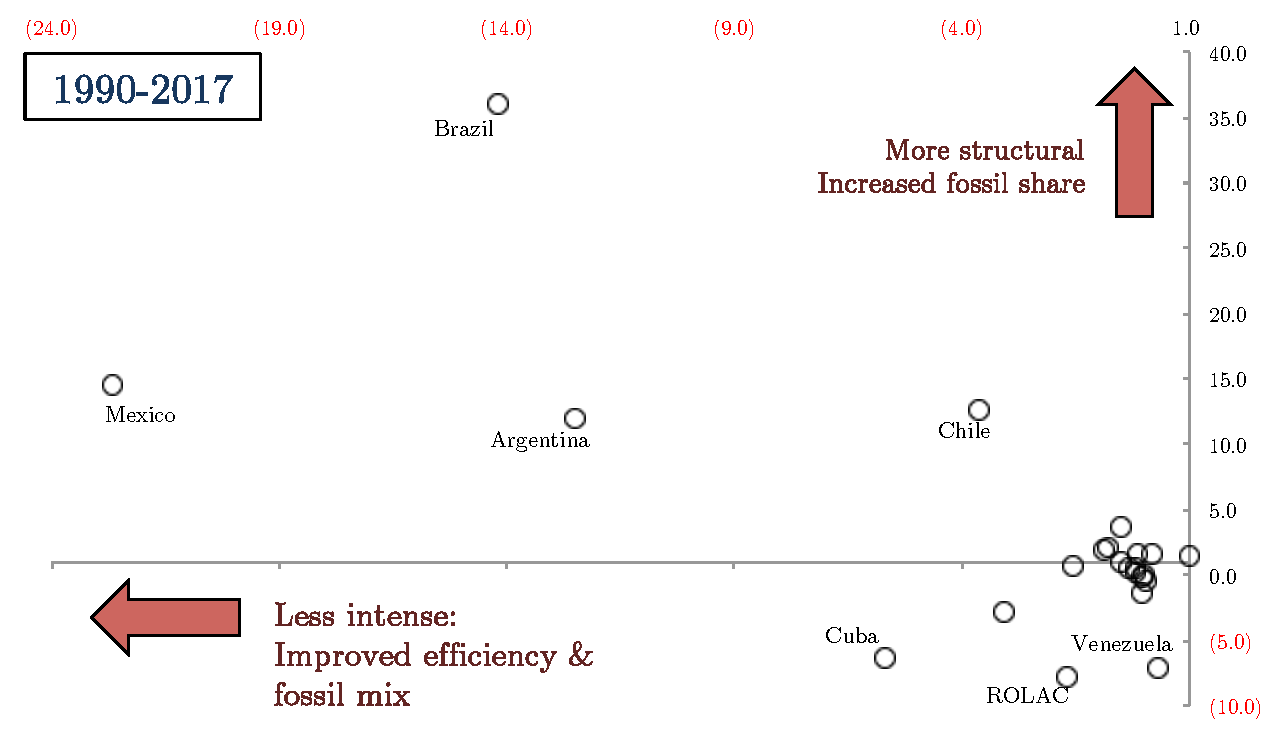
\includegraphics[width=11cm]{images/scatter1.pdf}
		\caption{LMDI analysis applied to  $CO_2$ emissions by country, period 1990-2017} 
		\label{countriesPlot}
	\end{center} 
\end{figure}

From intensity viewpoint, in general all countries become less intense (almost all intensity drivers are negative). This implies an overall improvement on efficiency and fuel-mix. Best improvements in efficiency and a more decarbonized fuel-mix is observed in Mexico, Brazil and Argentina. 
From structural viewpoint, Venezuela and Cuba decreased their fossil-share in the electricity dispatch. Conversely, Brazil is showing the most important fossil-share of the region.


\subsubsection{Period 1990-1995}

In the period (1990-1995) the ACI reduction observed (-6.9 \%) is described by changes in intensity ($\Delta V_{int}$=-14.1 gCO$_2$/kWh) in specific due to the improvement of efficiency ($\Delta V_{u}$=-4.7 gCO$_2$/kWh) mainly associated with integration
of more efficient gas-fired plants ($\Delta V_{u2}$=-4.7 gCO$_2$/kWh) in Argentina. It is worth to note that structural drivers also explain the decrease of the ACI ($\Delta V_{p}$=-4.5 gCO$_2$/kWh) due to integration of large hydro resources in Venezuela.  During this lapse improvements both in structure and intensity were observed.

\subsubsection{Period 1995-2003}

In the period (1995-2003) the ACI increase observed (11.0 \%) is described by changes in structure ($\Delta V_{str}$ = 48.6 gCO$_2$/kWh) in specific due to an increased fossil-share of electricity output ($\Delta V_{p}$ = 40.7 gCO$_2$/kWh) mainly associated with integration of  fossil fuel-fired plants in Mexico and Brazil.

\subsubsection{Period 2003-2008}

In the period (2003-2008) the ACI reduction observed (-9.1 \%) is explained by changes in intensity ($\Delta V_{int}$ = -28.4 gCO$_2$/kWh) in specific due to the improvement of efficiency ($\Delta V_{u}$ = -16.0 gCO$_2$/kWh) mainly associated with the modernization of fuel oil thermal plants ($\Delta V_{u3}$ = -9.2 gCO$_2$/kWh) in Mexico.

\subsubsection{Period 2008-2015}

In the period (2008-2015) the ACI increase observed (17.1 \%) is described by changes in structure ($\Delta V_{str}$ = 34.8 gCO$_2$/kWh) in specific due to an increased fossil-share of electricity output ($\Delta V_{p}$ = 35.4 gCO$_2$/kWh). The main actor is Brazil with large integration
of  fossil fuel-fired plants.

\subsubsection{Period 2015-2017}

In the period (2015-2017) the ACI reduction observed (-9.9 \%) is described by changes in bot intensity ($\Delta V_{int}$ = -9.2 gCO$_2$/kWh) and structure ($\Delta V_{str}$ = -18.2 gCO$_2$/kWh). Intensity effects were characterized by the improvement of efficiency ($\Delta V_{u}$ = -10.6 gCO$_2$/kWh) in Argentina and Brazil. It is worth to note that structural drivers also explain the decrease of the ACI ($\Delta V_{p}$ = -18.4 gCO$_2$/kWh) due to a decrease of the fossil share in Brazil. Figure \ref{countriesPlots} shows the changes of ACI total, intensity and structural by country for the period 2015-2017.  

\subsubsection{Period 2015-2017}
        \begin{figure}[H]
	\begin{center} 
		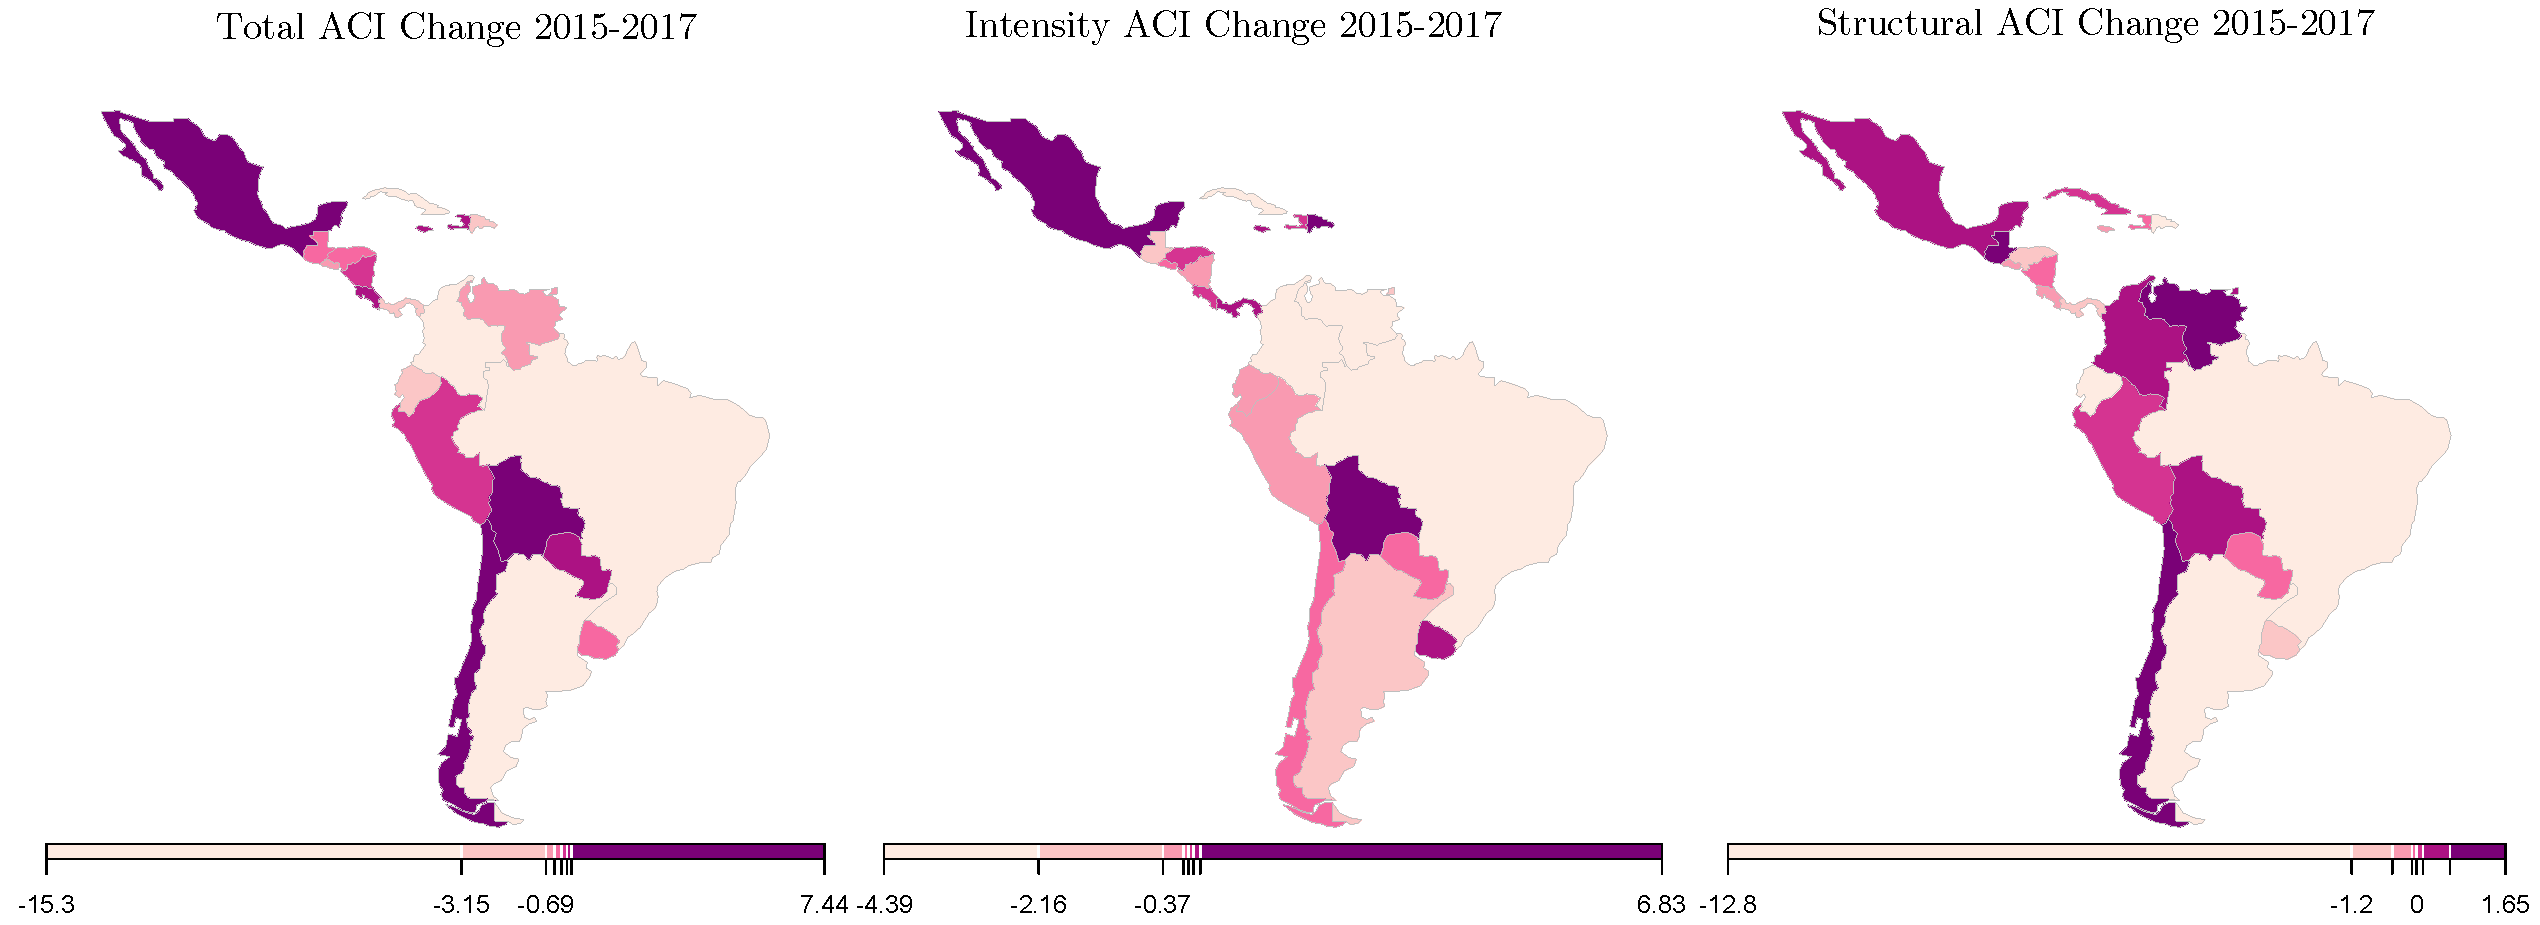
\includegraphics[width=15.6cm]{images/Rplot_1517.pdf}
		\caption{LMDI analysis applied to  $CO_2$ emissions by country, period 2015-2017} 
		\label{countriesPlots}
	\end{center} 
\end{figure}

\subsection{The Multiplicative IDA-LMDI analysis results}

Another method to decompose the relative change of the ACI is the multiplicative decomposition model presented in Section \ref{amm2}. In this representation the change of the ACI is given as a proportion of the base year value. For instance, the total change is $\Delta V$=2.1 gCO$_2$/kWh in additive form but in its multiplicative form, the change of the ACI is now represented as $ U$=0.9917. Therefore, each decomposed structural and intensity factor is given as a proportion the base value.
Hence the additive and multiplicative
decomposition results can be confirmed with each other. The multiplicative approach is convenient to confirm the results obtained in section \ref{addres} using a suitable graphical representation.

  Figure  \ref{main6} shows a pictorial view of the ACI decomposition factors in multiplicative form for the period 1990-2017.

 

            \begin{figure}[!ht] \centerline{
     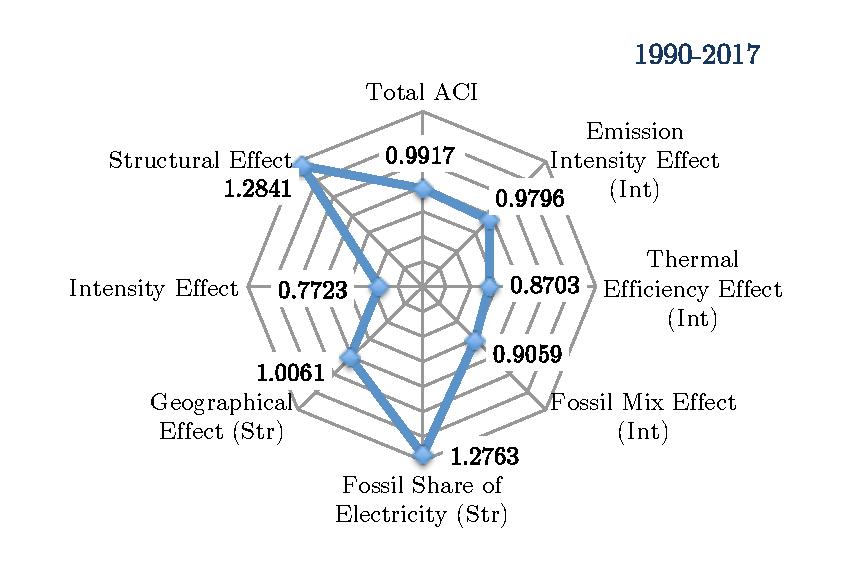
\includegraphics[width=11cm]{images/main6.pdf}}
       \caption{Pictorial view of the ACI decomposition factors for the period 1990-2017}
      \label{main6}
        \end{figure}


The multiplicative decomposition approach confirms that intensity effect ($U_{int}$=0.7723) is main the driving force behind the decrease of the ACI in Latin America and the Caribbean countries between 1990 and 2017 ($U$=0.9917). The intensity effect reveals an important mitigating effect being the fossil fuel-mix ($U_{m}$=0.9059) and the thermal efficiency ($U_{u}$=0.8703) the most important intensity effects. The structural change is $U_{str}$=1.2841. The main structural effect is the increasing fossil-share of electricity output ($U_{p}$=1.2763). Note that the geographical shift factor ($U_{s}$=1.0161) and CO$_2$ emission factors ($U_{e}$=0.9796) are not relevant.

 
         \begin{figure}[!ht] \centerline{
     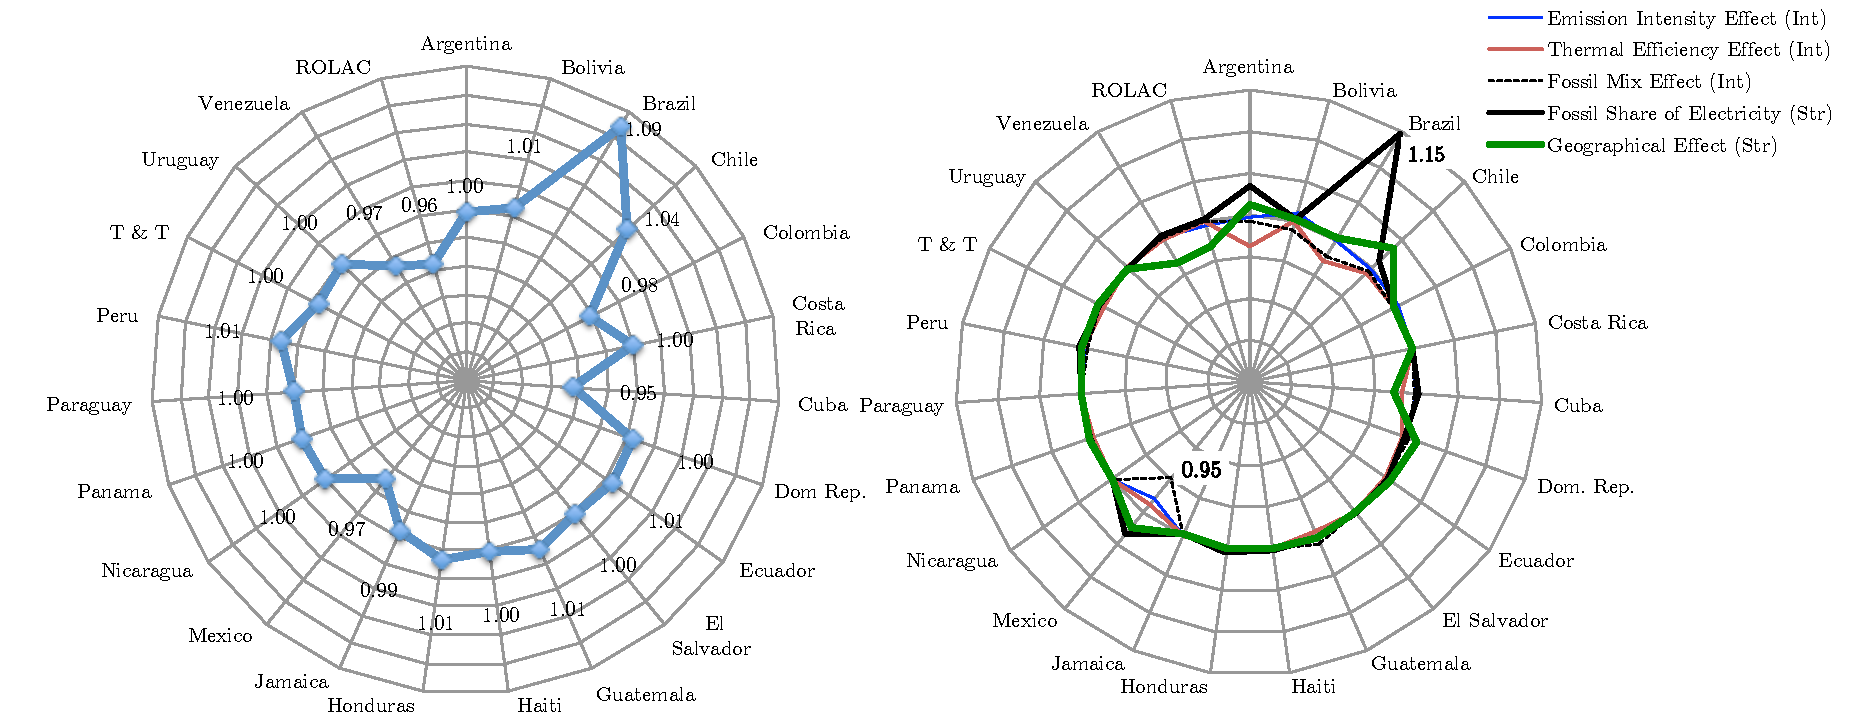
\includegraphics[width=16cm]{images/main11.pdf}}
       \caption{Pictorial view of the ACI decomposition factors for the period 1990-2017 - Results by Country}
      \label{main5}
        \end{figure}

  Figure  \ref{main5} shows a pictorial view of the ACI decomposition factors by country.  Fairly substantial increase is observed in Brazil. The structural factor fossil-share of electricity  $U^{bra}_{p}$ is the highest (1.15). Figure \ref{main5} also shows the important role of Mexico with a fossil-mix effect of $U^{mex}_{m}$ of 0.95.  Both results confirm the  analyses previously  summarized in section \ref{addres}.
 
 \section{The future of carbon intensity in Latin America}  \label{policy}

 Figure \ref{ACI2}
shows the historical evolution of the carobon intensity between 1990 and 2017 and two forecasted scenarios provided by the International Energy Agency for 2017-2040 \citep{weio2014}.  

  \begin{figure}[ht] \centerline{
     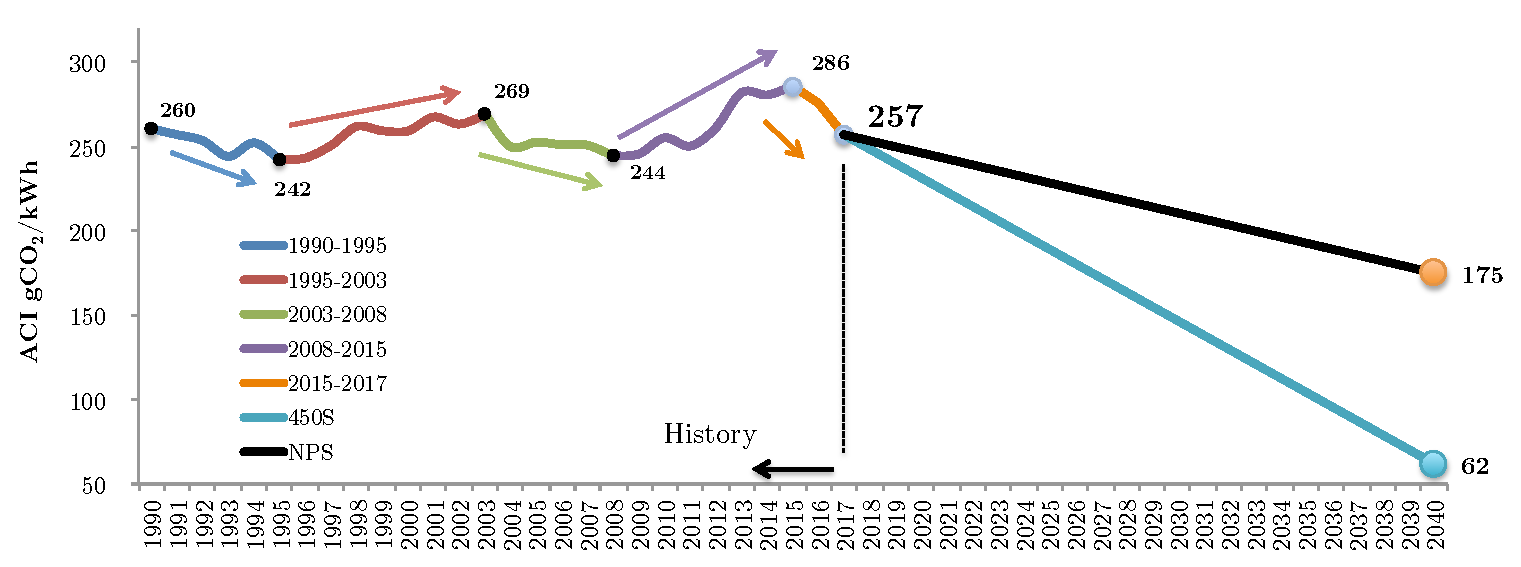
\includegraphics[width=12cm]{images/LACACIf.pdf}}
       \caption{Aggregate carbon intensity of electricity in LAC countries (1990-2017) and IEA's NPS and 450S forecasts (2017-2040),  \citep{weio2014}}
      \label{ACI2}
        \end{figure}


Note that in during 1990-1995 and 2003-2008 periods, LAC countries were able to reduce their carbon intensity almost 5 \%. However, in recent years this index has increased almost 15 \% changing from 244 gCO$_2$/kWh in 2008 to 286 gCO$_2$/kWh in 2015. However, since 2015 the carbon intensity decreased almost 9.1 \% to reach 257.7 gCO$_2$/kWh in 2017.

The future evolution of future CO$_2$ emissions might take different ways depending on the mitigation policy adopted. Figure \ref{ACI2} also depicts two future projections for LAC's ACI provided by the IEA. Under the New Policies Scenario \footnote{New Policies Scenario is the IEA baseline scenario. It takes account of broad policy commitments and plans that have been announced by LAC countries, including national pledges to reduce greenhouse-gas emissions and plans to phase out fossil-energy subsidies, even if the measures to implement these commitments have yet to be identified or announced.} (NPS), it is expected a reduction of 39 \% (from 286 gCO$_2$/kWh in 2017 to 175 gCO$_2$/kWh in 2040). Under the sustainable development scenario (450S) a strong decrease of 79 \% is also expected (from 286 gCO$_2$/kWh  in 1990 to 61 gCO$_2$/kWh in 2040). Then, both scenarios are showing a clear declining trend. The historical trend observed in 2015-2017 is aligned with both future scenarios. However, the accomplishment of the sustainable development goal (61 gCO$_2$/kWh in 2040) will require additional efforts from intensity and structural perspectives.


\section{Conclusions} \label{sec7}
 
 This paper analyzes the drivers behind the changes of the Aggregate Carbon Intensity (ACI) for electricity of Latin America \& the Caribbean (LAC) in five periods between 1990 and 2017. The conclusions are the following:
 \begin{itemize}
  \item 1990-2017 the ACI changed (decreased) from 259.8 to 257.7 gCO$_2$/kWh due to INTENSITY reasons (improvements in  gas-fired plant efficiency).
  \item 1990-1995 the ACI changed (decreased) from 259.8 to 242.1 gCO$_2$/kWh due to INTENSITY reasons (improvements in  fuel-fired plant efficiency).
  \item 1995-2003 the ACI changed (increased) from 242.1 to 263.8 gCO$_2$/kWh due to STRUCTURAL reasons (fossil-share increase)
  \item 2003-2008 the ACI changed (decreased) from 263.8 to 244.0 gCO$_2$/kWh due to INTENSITY reasons (improvements in  coal-fired plant efficiency).
  \item 2008-2015   the ACI changed (increased) from 244.0 to 286.0 gCO$_2$/kWh due to STRUCTURAL reasons (fossil-share increase)
  \item 2015-2017 when the ACI changed (decreased) from 286.0 to 257.7 gCO$_2$/kWh  due to INTENSITY reasons (improvements in  coal-fired plant efficiency and decrease of fossil-share).
\end{itemize}
 
 The historical trend observed in 2015-2017 is aligned with the sustainable development scenario required to achieve climate goals. However, current carbon intensity (257.7 gCO$_2$/kWh) is far from the sustainable development goal (62 gCO$_2$/kWh). Therefore, it is  required additional mitigating efforts from intensity and structural perspectives.

 
 
\reftitle{References}
\begin{thebibliography}{1}

\bibitem{WMO}  
World Meteorological Organization. \textit{WMO Greenhouse Gas Bulletin (GHG Bulletin)- No. 14: The State of Greenhouse Gases in the Atmosphere Based on Global Observations through 2017}, 2017. Available at https://library.wmo.int/  

\bibitem{2007IPCC}   Intergovernmental Panel on Climate Change.  Climate change 2007 synthesis report. Technical report contribution of working
groups I, II and III to the fourth assessment report of the Intergovernmental Panel
on Climate Change; 2007.

 


 \bibitem{IEAEnergyCombution2019} \textit{CO2 Emissions from Fuel Combustion}, International Energy Agency, Paris, 2019.

 \bibitem{weio2014} \textit{World Energy Investment Outlook}, International Energy Agency, 2014.

\bibitem{ang2016}  Ang, B. W.,  Su, B. (2016). Carbon emission intensity in electricity production: A global analysis. Energy Policy, 94, 56-63.





% CO2 ANALYSES

\bibitem{zhang2000}  Ang, B.W.,Zhang,F.Q.,2000. A survey of index decomposition analysis in energy
and environmental studies. Energy 25, 1149-1176.

\bibitem{xu2013}  Xu,X.Y.,Ang,B.W.,2013. Index decomposition analysis applied to CO2 emission
studies. Ecol.Econ. 93, 313-329.

\bibitem{jiang} Jiang, X. T., \& Li, R. (2017). Decoupling and Decomposition Analysis of Carbon Emissions from Electric Output in the United States. Sustainability, 9(6), 886.


\bibitem{zhao}  Zhao, Y., Li, H., Zhang, Z., Zhang, Y., Wang, S., \& Liu, Y. (2017). Decomposition and scenario analysis of CO2 emissions in China's power industry: based on LMDI method. Natural Hazards, 86(2), 645-668.


\bibitem{zkar} Karmellos, M., Kopidou, D., \& Diakoulaki, D. (2016). A decomposition analysis of the driving factors of CO2 (Carbon dioxide) emissions from the power sector in the European Union countries. Energy, 94, 680-692.

\bibitem{sum} Sumabat, A. K., Lopez, N. S., Yu, K. D., Hao, H., Li, R., Geng, Y., \& Chiu, A. S. (2016). Decomposition analysis of Philippine CO2 emissions from fuel combustion and electricity generation. Applied Energy, 164, 795-804.


\bibitem{dia} Diakoulaki, D., Giannakopoulos, D., \& Karellas, S. (2017). The driving factors of CO2 emissions from electricity generation in Greece: an index decomposition analysis. International Journal of Global Warming, 13(3-4), 382-397.

% ACI ANALYSES

\bibitem{goh} Ang BW, Goh T. (2016). Carbon intensity of electricity in ASEAN: drivers, performance and outlook. Energy Policy 2016;98:170-9.

\bibitem{peng} Peng, X., \& Tao, X. (2018). Decomposition of carbon intensity in electricity production: Technological
innovation and structural adjustment in china's power sector. Journal of Cleaner Production, 172, 805-818. 

\bibitem{liu} Liu, N., Ma, Z., \& Kang, J. (2017). A regional analysis of carbon intensities of electricity generation in China. Energy Economics, 67, 268-277.

 \bibitem{liu2} Liu, N., Ma, Z., Kang, J., \& Su, B. (2019). A multi-region multi-sector decomposition and attribution
analysis of aggregate carbon intensity in china from 2000 to 2015. Energy Policy, 129, 410-421. 

\bibitem{oliv} De Oliveira De Jesus, P. (2019). Effect of generation capacity factors on carbon emission intensity of electricity of Latin America and the Caribbean, a temporal ida-lmdi analysis. Renewable and
Sustainable Energy Reviews, 101, 516-526.   


\bibitem{angperfect}  Ang, B. W., Liu, F. L., \& Chew, E. P. (2003). Perfect decomposition techniques in energy and environmental analysis. Energy Policy, 31(14), 1561-1566.



 \bibitem{PDE} Ministry of Mines and Energy of Brazil (MME), Electricity in the 2024 Brazilian
Energy Plan (PDE 2024), Available at http://www.mme.gov.br/


\bibitem{EIA2013} EIA, International Energy Outlook. US Energy Information Administration. DOE/EIA-0484, 2013


% \bibitem{IEAWeo2016} IEA, 2016, International Energy Agency IEA. World Energy Outlook. OECD/IEA,
%9 rue de la Fédération 75739 Paris Cedex 15, France, 1st edition, 2016
%
%
% \bibitem{1} Ang, B.W., Zhou, P., Tay, L.P., 2011. Potential for reducing global carbon emissions
%from electricity production - a benchmarking analysis. Energy Policy 39,
%2482-2489.
%
%
%
%
% \bibitem{2} Herrmann, J.K., Savin, I., 2017. Optimal policy identification: insights from the
%German electricity market. Technol. Forecast. Soc. Change 122, 71-90.
%
%
% \bibitem{3}  Yan, Q., Zhang, Q., Zou, X., 2016. Decomposition analysis of carbon dioxide emissions
%in China's regional thermal electricity generation, 2000-2020. Energy
%112, 788e794.
%
% \bibitem{4}  Zha, D., Zhou, D., Ding, N., 2012. The determinants of aggregated electricity intensity
%in China. Appl. Energy 97, 150-156.
%
% \bibitem{5} Xu, P.,  Xiaoma, T. (2017). Decomposition of Carbon Intensity in Electricity Production: Technological Innovation and Structural Adjustment in China's Power Sector. Journal of Cleaner Production.
%
%\bibitem{6} Fernandez Gonzalez, P.,Moreno, B., 2016. Analyzing driving forces behind changes in energy vulnerability of Spanish electricity generation through a Divisia index-based method. Energy Convers. Manag. 92, 459-486.
%
% \bibitem{IEAEnergyCombution2012} IEA,2012, CO2 Emissions from Fuel Combustion, International Energy Agency, Paris, 2012.
% \bibitem{IEAEnergyCombution2013} IEA,2013, CO2 Emissions from Fuel Combustion, International Energy Agency, Paris, 2013.
% \bibitem{IEAEnergyCombution2014} IEA,2014, CO2 Emissions from Fuel Combustion, International Energy Agency, Paris, 2014.
% \bibitem{IEAEnergyCombution2016} IEA,2016, CO2 Emissions from Fuel Combustion, International Energy Agency, Paris, 2016.
% \bibitem{IEAEnergyCombution2016} IEA,2016a, CO2 Emissions from Fuel Combustion, International Energy Agency, Paris, 2016.
% \bibitem{IEAEnergyCombution2016} IEA,2016, CO2 Emissions from Fuel Combustion, International Energy Agency, Paris, 2016.
% \bibitem{IEAEnergyCombution2017} IEA,2017, CO2 Emissions from Fuel Combustion, International Energy Agency, Paris, 2016.
%
% \bibitem{IEABalances2016} IEA, 2016b, International Energy Agency,  Energy Balances of OECD/Non-OECD Countries, Paris. On-line: https://www.iea.org/statistics/
%statisticssearch/.
%
%
% \bibitem{10} Malla, S., 2009. CO2 emissions from electricity generation in seven Asia-Pacific and
%North American countries: a decomposition analysis. Energy Policy 37, 1-9.
%
%\bibitem{11} Ang, B.W., 2005. The LMDI approach to decomposition analysis: a practical guide.
%Energy Policy 33, 867-871.
%
%\bibitem{12} Maruyama, N., Eckelman, M.J.,2009. Longterm trends of electric efficiencies in
%electricity generation in developing  countries. Energy Policy 37,1678-1686
%
%\bibitem{13} Graus, W., Worrell, E.,2009. Trend in efficiency and capacity of fossil power
%generation in the EU.Energy Policy 37, 2147-2160.
%


%
%\bibitem{Ilic}
%Rotering, N.; Ilic, M.  Optimal charge control of plug-in hybrid electric vehicles in deregulated electricity markets. {\em IEEE Trans. Power Syst.} {\bf2011}, {\em 26}, 1021--1029.
%
%\bibitem{Deb}
%Deb, S.; Tammi, K.; Kalita, K.; Mahanta, P.  Impact of Electric Vehicle Charging Station Load on Distribution Network. {\em Energies} {\bf2018}, {\em11}, 178.
%
%\bibitem{Bessa}
%Bessa, R.J.; Matos, M.A. Economic and technical management of an aggregation agent for electric vehicles: A~literature survey. {\em Int. Trans.  Electr. Energy Syst.} {\bf2012} {\em22}, 334--350.
%
%\bibitem{Zhang}
%Zhang, Z.J.; Nair, N.C. Economic and pricing signals in electricity distribution systems: A~bibliographic survey. In {Proceedings of the}{ IEEE International Conference on Power System Technology (POWERCON)}, Auckland, New Zealand,  30 October--2 November 2012; pp. 1--6.
%
%
%\bibitem{Pan}
%Pan, J.; Teklu, Y.; Rahman, S.;  Jun, K. Review of usage-based transmission cost allocation methods under open access.  {\em IEEE Trans. Power Syst.} {\bf2000}, {\em 15}, 1218--1224.
%
%
%\bibitem{Carpaneto}
%Carpaneto, E.; Chicco, G.; Akilimali, J.S. Characterization of the loss allocation techniques for radial systems
%with distributed generation. {\em Electr. Power Syst. Res}. {\bf2008}, {\em78}, 1396--1406.
%



\end{thebibliography}


\appendix

\section{Decomposition IDA-LMDI formulae for the additive approach}\label{app1}


The decomposition IDA-LMDI formulae for the additive approach is included below:

\begin{equation}\label{dvtot1}
  \Delta V_{e}   = \sum^n_{j=1} \sum^f_{i=1}   L(w_{ij}^{t_f},w_{ij}^{t_0}) \ln(\frac{e^{t_f}_{ij}}{e^{t_0}_{ij}})
\end{equation}
\begin{equation}\label{dvtot2}
  \Delta V_{u}   = \sum^n_{j=1} \sum^f_{i=1}   L(w_{ij}^{t_f},w_{ij}^{t_0}) \ln(\frac{u^{t_f}_{ij}}{u^{t_0}_{ij}})
\end{equation}

\begin{equation}\label{dvtot3}
  \Delta V_{m}   = \sum^n_{j=1} \sum^f_{i=1}   L(w_{ij}^{t_f},w_{ij}^{t_0}) \ln(\frac{m^{t_f}_{j}}{m^{t_0}_{j}})
\end{equation}

\begin{equation}\label{dvtot4}
  \Delta V_{p}   = \sum^n_{j=1} \sum^f_{i=1}   L(w_{ij}^{t_f},w_{ij}^{t_0}) \ln(\frac{p^{t_f}_{j}}{p^{t_0}_{j}})
\end{equation}

\begin{equation}\label{dvtot5}
  \Delta V_{s}   = \sum^n_{j=1} \sum^f_{i=1}   L(w_{ij}^{t_f},w_{ij}^{t_0}) \ln(\frac{s^{t_f}_{j}}{s^{t_0}_{j}})
\end{equation}

where $w^{t_f}_{ij}=\frac{C^{t_f}_{ij}}{G^{t_f}}$, $w^{t_0}_{ij}=\frac{C^{t_0}_{ij}}{G^{t_0}}$ and
$L(a,b)=\frac{a-b}{\ln{a}-\ln{b}}$


\section{Decomposition IDA-LMDI formulae for the multiplicative approach}\label{app2}

The decomposition IDA-LMDI formulae for the multiplicative approach is included below:

\begin{equation}
  U_{e}   = e^{\sum^n_{j=1}\sum^f_{i=1}
  \frac{L(w_{ij}^{t_f},w_{ij}^{t_0})} {L(V^{t_f},V^{t_0})}\ln(\frac{e^{t_f}_{j}}{e^{t_0}_{j}})}
\end{equation}
\begin{equation}
  U_{u}   = e^{\sum^n_{j=1} \sum^f_{i=1}
  \frac{L(w_{ij}^{t_f},w_{ij}^{t_0})} {L(V^{t_f},V^{t_0})}\ln(\frac{u^{t_f}_{j}}{u^{t_0}_{j}})}
\end{equation}
\begin{equation}
  U_{m}   = e^{\sum^n_{j=1}\sum^f_{i=1}
  \frac{L(w_{ij}^{t_f},w_{ij}^{t_0})} {L(V^{t_f},V^{t_0})}\ln(\frac{m^{t_f}_{j}}{m^{t_0}_{j}})}
\end{equation}
\begin{equation}
  U_{p}   = e^{\sum^n_{j=1}\sum^f_{i=1}
  \frac{L(w_{ij}^{t_f},w_{ij}^{t_0})} {L(V^{t_f},V^{t_0})}\ln(\frac{p^{t_f}_{j}}{p^{t_0}_{j}})}
\end{equation}
\begin{equation}
  U_{s}   = e^{\sum^n_{j=1} \sum^f_{i=1}
  \frac{L(w_{ij}^{t_f},w_{ij}^{t_0})} {L(V^{t_f},V^{t_0})}\ln(\frac{s^{t_f}_{j}}{s^{t_0}_{j}})}
\end{equation}
where $w^{t_f}_{j}=\frac{C^{t_f}_{j}}{G^{t_f}}$, $w^{t_0}_{j}=\frac{C^{t_0}_{j}}{G^{t_0}}$ and
$L(a,b)=\frac{a-b}{\ln{a}-\ln{b}}$



%\section{Latin American countries energy and emissions database }\label{app3}
%
%
%       \begin{table}[H] \centerline{
%     \includegraphics[width=15cm]{images/database.pdf}}
%       \caption{Energy and emissions database for LAC countries (1990-2017)}
%      \label{database2}
%        \end{table}






%\section{Additive IDA-LMDI Results by Country 1990-2017}\label{app4}



%Table \ref{table3} presents the results of the additive IDA-LMDI decomposition by country for the period 1990-2017.



\section{Multiplicative IDA-LMDI Results by Country 1990-2017}\label{app4}

Table \ref{table4} presents the results of the multiplicative IDA-LMDI decomposition by country for the period 1990-2017.

  \begin{table}[!h]\label{11}										
\begin{center}\caption{Proportional Change on ACI (1990-2017) - Results by Country}			
\begin{tabular}{l|c|c:c|ccc:cc}\hline	
Country	&$	U_{tot}	$&$	U_{int}	$&$	U_{str}	$&$	U_e	$&$	U_u	$&$	U_m	$&$	U_p	$&$	U_s$	\\\hline
 Argentina 	 & 	0.9980 	 & 	0.9529 	&	1.0474 	&	0.9969 	&	0.9621 	&	0.9935 	&	1.0344 	&	1.0126 	\\
 Bolivia 	 & 	1.0059 	 & 	0.9995 	&	1.0064 	&	1.0107 	&	1.0000 	&	0.9889 	&	1.0030 	&	1.0034 	\\
 Brazil 	 & 	1.0880 	 & 	0.9466 	&	1.1494 	&	0.9993 	&	0.9697 	&	0.9768 	&	1.1470 	&	1.0020 	\\
 Chile 	 & 	1.0352 	 & 	0.9861 	&	1.0497 	&	0.9994 	&	0.9921 	&	0.9946 	&	1.0135 	&	1.0358 	\\
 Colombia 	 & 	0.9773 	 & 	0.9883 	&	0.9889 	&	1.0002 	&	0.9944 	&	0.9937 	&	0.9950 	&	0.9939 	\\
 Costa Rica 	 & 	0.9996 	 & 	0.9998 	&	0.9997 	&	0.9999 	&	1.0000 	&	1.0000 	&	0.9997 	&	1.0000 	\\
 Cuba 	 & 	0.9549 	 & 	0.9783 	&	0.9761 	&	0.9991 	&	0.9817 	&	0.9975 	&	1.0029 	&	0.9732 	\\
 Dom. Rep. 	 & 	1.0043 	 & 	0.9967 	&	1.0077 	&	0.9997 	&	0.9943 	&	1.0027 	&	0.9952 	&	1.0125 	\\
 Ecuador 	 & 	1.0051 	 & 	0.9971 	&	1.0080 	&	0.9998 	&	0.9979 	&	0.9994 	&	1.0029 	&	1.0051 	\\
 El Salvador 	 & 	1.0012 	 & 	0.9994 	&	1.0019 	&	1.0001 	&	0.9993 	&	1.0000 	&	1.0019 	&	0.9999 	\\
 Guatemala 	 & 	1.0095 	 & 	1.0038 	&	1.0056 	&	0.9998 	&	0.9939 	&	1.0101 	&	1.0034 	&	1.0022 	\\
 Haiti 	 & 	1.0009 	 & 	0.9988 	&	1.0021 	&	1.0001 	&	0.9988 	&	1.0000 	&	1.0028 	&	0.9993 	\\
 Honduras 	 & 	1.0068 	 & 	1.0007 	&	1.0062 	&	1.0000 	&	1.0003 	&	1.0003 	&	1.0054 	&	1.0008 	\\
 Jamaica 	 & 	0.9947 	 & 	0.9999 	&	0.9948 	&	1.0008 	&	0.9991 	&	1.0000 	&	0.9980 	&	0.9968 	\\
 Mexico 	 & 	0.9694 	 & 	0.9162 	&	1.0580 	&	0.9785 	&	0.9882 	&	0.9476 	&	1.0339 	&	1.0233 	\\
 Nicaragua 	 & 	1.0002 	 & 	0.9992 	&	1.0010 	&	1.0000 	&	0.9992 	&	1.0000 	&	1.0006 	&	1.0004 	\\
 Panama 	 & 	1.0022 	 & 	0.9981 	&	1.0041 	&	0.9998 	&	0.9981 	&	1.0002 	&	1.0024 	&	1.0017 	\\
 Paraguay 	 & 	1.0000 	 & 	1.0000 	&	1.0000 	&	1.0000 	&	1.0000 	&	1.0000 	&	1.0000 	&	1.0000 	\\
 Peru 	 & 	1.0123 	 & 	0.9981 	&	1.0143 	&	0.9993 	&	1.0019 	&	0.9969 	&	1.0084 	&	1.0059 	\\
 T \& T 	 & 	0.9965 	 & 	0.9940 	&	1.0025 	&	1.0000 	&	0.9940 	&	1.0000 	&	1.0001 	&	1.0024 	\\
 Uruguay 	 & 	0.9985 	 & 	1.0001 	&	0.9983 	&	1.0001 	&	1.0001 	&	1.0000 	&	0.9987 	&	0.9996 	\\
 Venezuela 	 & 	0.9741 	 & 	1.0013 	&	0.9729 	&	1.0027 	&	0.9976 	&	1.0010 	&	1.0047 	&	0.9683 	\\
 ROLAC 	 & 	0.9643 	 & 	0.9935 	&	0.9706 	&	0.9935 	&	1.0000 	&	1.0000 	&	1.0013 	&	0.9693 	\\\hline
Total	 & 	0.9917 	 & 	0.7723 	&	1.2841 	&	0.9796 	&	0.8703 	&	0.9059 	&	1.2763 	&	1.0061 		
\end{tabular}	\label{table4}									
\end{center}										
\end{table}	




\end{document}
